% Chapter 3
\glsresetall % reset the glossary to expand acronyms again
\chapter{Prototype Implementation}\label{ch:Prototype}

In order to validate the claims of simplicity and feasibility, a prototype
implementation of the Garter language was devised, and some example
programs were written in Garter.

The prototype was built by modifying the cpython compiler \cite{cpython} and
tooling to support the extra functionality provided by Garter, and then adding a
validation pass using the extra functionality to ensure correctness of the
Garter code.

Many options were considered for how to implement this prototype, mostly
focusing on Garter's similarity to Python, parsing and validating the program,
and then generating finished Python logic. See
Appendix \ref{ch:ExamplePrograms}.

\section{Program Structure}

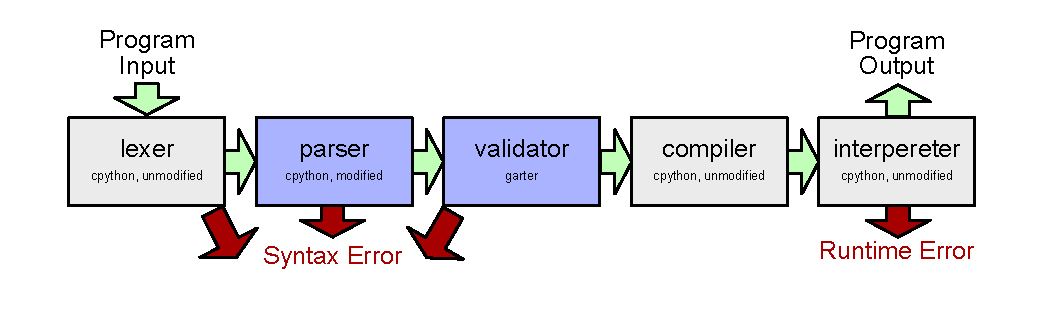
\includegraphics[width=\textwidth]{figs/proto_design.pdf}
% cpython (lexer) -> cpython (parser) -> garter (validator) -> cpython (compiler) -> cpython (interpereter) (DIAGRAM)

The Garter prototype implementation consisted of two major changes. Firstly, the
cpython parser and AST was extended to support the \code{:=} and \code{: T =}
declaration syntax. This was handled by adding an optional property on the
Assignment statement which indicates whether it is a declaration, and what type
was written. Types in the AST are represented as expressions, for backwards
compatibility with Python's PEP 3107 -- Function
Annotations \cite{pythonfuncannot}. The parser was then modified to accept the
extra syntax, and represent it correctly in the AST. The lexer, compiler, and
interpereter were left unmodified, such that Python code, some of which is
essential to the operation of cpython's logic, would continue to function
correctly.

A validation pass was then written. This pass operates on the AST objects
created by the parser, and performs the validation passes, type checking, and
other restrictions which Garter enforces on code written in it compared to
Python. This pass was written as a Python function in the \code{garter} module.
For ease of integration with existing tools in the Python ecosystem, the entry
point was given the same signature as Python's built-in \code{compile} function.
It acts like \code{compile}, except performs the validation first.

The entry points for interacting with Python were then also modified. The IDLE
IDE provided by Python was modified such that code compilation was dispatched
through Garter's \code{gcompile} function, rather than through the default
compile framework, meaning that typechecking functions correctly. In addition,
the Python \code{code} module was updated to also dispatch through \code{gcompile},
meaning that a command-line garter interpereter is also avaliable through the
command \code{./python -m gcode}. This program acts similarially to the default
Python executable. It is, however, not the default action right now in order to
not break the build process. The relatively minor amount of extra work to make
this the default code path is an important step.

The decision to insert the extra validation phase only when explicitly compiling
garter code, rather than simply modifying the default \code{compile} infrastructure,
was made in order to not break the rest of Python. cpython depends on large amounts
of Python code internally, which would be broken by the Garter validation passes.
Instead, just the major entry points for new developers were changed over, with
normal Python code still being run internally.

\section{REPL Support}

One of the useful properties of Python for teaching is it's support for a
Read-Eval-Print-Loop (REPL). REPLs help new programmers learn how their language
will behave by getting immediate responses for the behavior of program
fragments, and enabling experimentation. Some modifications had to be made to
the REPL environments, such as the one found in IDLE, in order to support the
validation phase needed by Garter. First, REPLs require maintaining scope and
type information across compilations. This was achieved by providing callers of
the \code{gcompile} API access to an opaque scope object which contains this
information. The callers had to be modified to retain this information across
calls to the \code{gcompile} API.

In addition, the callers had to be modified to roll-back the changes made to the
scope object if a runtime error occured during the execution of a program
fragment, as a runtime error could cause new declarations to not be initialized.
This required slightly more extensive changes to the call sites, however it was
not too complex to re-purpose the existing infrastructure for this purpose.

